\chapter{有向グラフ - Directed graphs}

ここでは2つの特徴を持つグラフについて検討していきます。
\begin{itemize}
\item \key{非巡回グラフ - Acyclic graphs}:
閉路を含まない有向グラフのこと。時にDAG(Directed Acyclic Graphs)と呼ばれる
\item \key{Successor graphs}:
各ノードの出次が1であるグラフ。このため、ただ一つの子を持つ。
\end{itemize}
どちらの場合も、グラフの特別な性質に基づく
効率的なアルゴリズムがあります。

\section{トポロジカルソート - Topological sorting}

\index{トポロジカルソート - topological sorting}
\index{閉路 - cycle}

\key{トポロジカルソート - topological sort}とは、
有向グラフのノードにおいて、ノード$a$からノー ド$b$へのパスが存在する場合、
ノードaがノードbの前に現れるような順序を持つグラフのことです。

\begin{center}
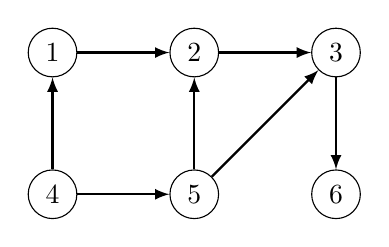
\begin{tikzpicture}[scale=0.9]
\node[draw, circle] (1) at (1,5) {$1$};
\node[draw, circle] (2) at (3,5) {$2$};
\node[draw, circle] (3) at (5,5) {$3$};
\node[draw, circle] (4) at (1,3) {$4$};
\node[draw, circle] (5) at (3,3) {$5$};
\node[draw, circle] (6) at (5,3) {$6$};

\path[draw,thick,->,>=latex] (1) -- (2);
\path[draw,thick,->,>=latex] (2) -- (3);
\path[draw,thick,->,>=latex] (4) -- (1);
\path[draw,thick,->,>=latex] (4) -- (5);
\path[draw,thick,->,>=latex] (5) -- (2);
\path[draw,thick,->,>=latex] (5) -- (3);
\path[draw,thick,->,>=latex] (3) -- (6);
\end{tikzpicture}
\end{center}
このトポロジカルソートは
$[4,1,5,2,3,6]$です。
\begin{center}
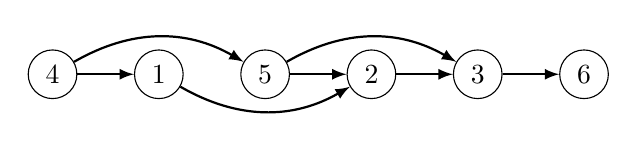
\begin{tikzpicture}[scale=0.9]
\node[draw, circle] (1) at (-6,0) {$1$};
\node[draw, circle] (2) at (-3,0) {$2$};
\node[draw, circle] (3) at (-1.5,0) {$3$};
\node[draw, circle] (4) at (-7.5,0) {$4$};
\node[draw, circle] (5) at (-4.5,0) {$5$};
\node[draw, circle] (6) at (-0,0) {$6$};

\path[draw,thick,->,>=latex] (1) edge [bend right=30] (2);
\path[draw,thick,->,>=latex] (2) -- (3);
\path[draw,thick,->,>=latex] (4) -- (1);
\path[draw,thick,->,>=latex] (4) edge [bend left=30] (5);
\path[draw,thick,->,>=latex] (5) -- (2);
\path[draw,thick,->,>=latex] (5) edge [bend left=30]  (3);
\path[draw,thick,->,>=latex] (3) -- (6);
\end{tikzpicture}
\end{center}

非巡回グラフは常にトポロジカルソートです。
しかし,グラフが閉路を含む場合は
閉路のどのノードも順序においてサイクルの他のノードより前に現れることができないので
トポロジカルソートを形成することはできません。
深さ優先探索を用いて,
有向グラフに閉路があるかどうかを調べ,
閉路がない場合にはトポロジカルソートを構成することができると判定できます。

\subsubsection{アルゴリズム - Algorithm}

ベースとなる考え方はグラフのノードを適当にみていき、
まだ処理されていない場合はそのノードから深さ優先探索を開始していきます。
ノードは3つのいずれかの状態を持ちます。

\begin{itemize}
\item 状態 0: ノードは処理されていない状態(白色)
\item 状態 1: ノードが処理中(薄いグレー)
\item 状態 2: ノードが処理された状態(濃いグレー)
\end{itemize}

初期状態では、各ノードの状態は0です。初めて検索が到達するとノードの状態は1になります。そして、そのノードのすべての探索が処理された後、そのノードの状態は2にします。

グラフに閉路が存在する場合、状態が1であるノードに探索をするので探索中にグラフに閉路があることが判明します。

グラフがサイクルを含まない場合はこの条件以外の時で、全てのノードの状態が2になったときに各ノードの探索順をリストとすることで、
トポロジカルソートとなります。

\subsubsection{Example 1}

このグラフの例では1,2,3,6と探索が進みます。

\begin{center}
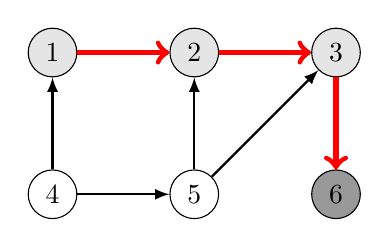
\begin{tikzpicture}[scale=0.9]
\node[draw, circle,fill=gray!20] (1) at (1,5) {$1$};
\node[draw, circle,fill=gray!20] (2) at (3,5) {$2$};
\node[draw, circle,fill=gray!20] (3) at (5,5) {$3$};
\node[draw, circle] (4) at (1,3) {$4$};
\node[draw, circle] (5) at (3,3) {$5$};
\node[draw, circle,fill=gray!80] (6) at (5,3) {$6$};

\path[draw,thick,->,>=latex] (4) -- (1);
\path[draw,thick,->,>=latex] (4) -- (5);
\path[draw,thick,->,>=latex] (5) -- (2);
\path[draw,thick,->,>=latex] (5) -- (3);
%\path[draw,thick,->,>=latex] (3) -- (6);

\path[draw=red,thick,->,line width=2pt] (1) -- (2);
\path[draw=red,thick,->,line width=2pt] (2) -- (3);
\path[draw=red,thick,->,line width=2pt] (3) -- (6);
\end{tikzpicture}
\end{center}

ここで、6には探索する先がないので、状態2となり、リストに値が登録されます。
次に、3,2,1と追加されていきます。

\begin{center}
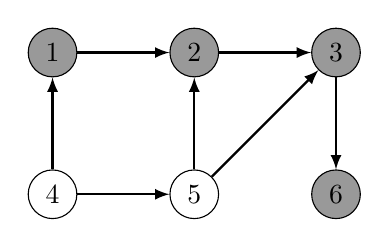
\begin{tikzpicture}[scale=0.9]
\node[draw, circle,fill=gray!80] (1) at (1,5) {$1$};
\node[draw, circle,fill=gray!80] (2) at (3,5) {$2$};
\node[draw, circle,fill=gray!80] (3) at (5,5) {$3$};
\node[draw, circle] (4) at (1,3) {$4$};
\node[draw, circle] (5) at (3,3) {$5$};
\node[draw, circle,fill=gray!80] (6) at (5,3) {$6$};

\path[draw,thick,->,>=latex] (1) -- (2);
\path[draw,thick,->,>=latex] (2) -- (3);
\path[draw,thick,->,>=latex] (4) -- (1);
\path[draw,thick,->,>=latex] (4) -- (5);
\path[draw,thick,->,>=latex] (5) -- (2);
\path[draw,thick,->,>=latex] (5) -- (3);
\path[draw,thick,->,>=latex] (3) -- (6);
\end{tikzpicture}
\end{center}

いま、リストの状態は$[6,3,2,1]$です。次は4が探索されます。

\begin{center}
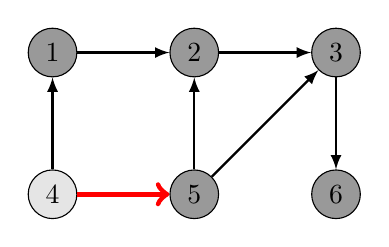
\begin{tikzpicture}[scale=0.9]
\node[draw, circle,fill=gray!80] (1) at (1,5) {$1$};
\node[draw, circle,fill=gray!80] (2) at (3,5) {$2$};
\node[draw, circle,fill=gray!80] (3) at (5,5) {$3$};
\node[draw, circle,fill=gray!20] (4) at (1,3) {$4$};
\node[draw, circle,fill=gray!80] (5) at (3,3) {$5$};
\node[draw, circle,fill=gray!80] (6) at (5,3) {$6$};

\path[draw,thick,->,>=latex] (1) -- (2);
\path[draw,thick,->,>=latex] (2) -- (3);
\path[draw,thick,->,>=latex] (4) -- (1);
%\path[draw,thick,->,>=latex] (4) -- (5);
\path[draw,thick,->,>=latex] (5) -- (2);
\path[draw,thick,->,>=latex] (5) -- (3);
\path[draw,thick,->,>=latex] (3) -- (6);

\path[draw=red,thick,->,line width=2pt] (4) -- (5);
\end{tikzpicture}
\end{center}

このようにリスト$[6,3,2,1,5,4]$を得ることができます。
この逆順がトポロジカルソート$[4,5,1,2,3,6]$です。

\begin{center}
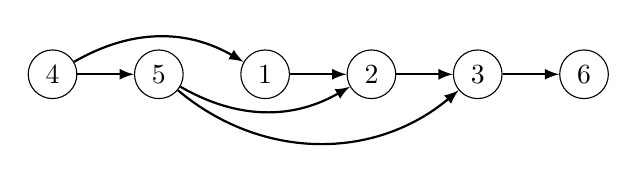
\begin{tikzpicture}[scale=0.9]
\node[draw, circle] (1) at (3,0) {$1$};
\node[draw, circle] (2) at (4.5,0) {$2$};
\node[draw, circle] (3) at (6,0) {$3$};
\node[draw, circle] (4) at (0,0) {$4$};
\node[draw, circle] (5) at (1.5,0) {$5$};
\node[draw, circle] (6) at (7.5,0) {$6$};

\path[draw,thick,->,>=latex] (1) -- (2);
\path[draw,thick,->,>=latex] (2) -- (3);
\path[draw,thick,->,>=latex] (4) edge [bend left=30] (1);
\path[draw,thick,->,>=latex] (4) -- (5);
\path[draw,thick,->,>=latex] (5) edge [bend right=30] (2);
\path[draw,thick,->,>=latex] (5) edge [bend right=40] (3);
\path[draw,thick,->,>=latex] (3) -- (6);
\end{tikzpicture}
\end{center}

なお、トポロジカルソートは1つとは限りません。
閉路を含まないグラフでは複数のトポロジカルソートが存在しえます。

\subsubsection{Example 2}

閉路を含むのでトポロジカルソートできない場合はどうなるでしょうか。

\begin{center}
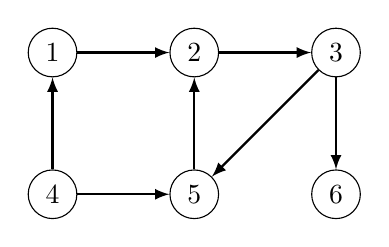
\begin{tikzpicture}[scale=0.9]
\node[draw, circle] (1) at (1,5) {$1$};
\node[draw, circle] (2) at (3,5) {$2$};
\node[draw, circle] (3) at (5,5) {$3$};
\node[draw, circle] (4) at (1,3) {$4$};
\node[draw, circle] (5) at (3,3) {$5$};
\node[draw, circle] (6) at (5,3) {$6$};

\path[draw,thick,->,>=latex] (1) -- (2);
\path[draw,thick,->,>=latex] (2) -- (3);
\path[draw,thick,->,>=latex] (4) -- (1);
\path[draw,thick,->,>=latex] (4) -- (5);
\path[draw,thick,->,>=latex] (5) -- (2);
\path[draw,thick,->,>=latex] (3) -- (5);
\path[draw,thick,->,>=latex] (3) -- (6);
\end{tikzpicture}
\end{center}
次のように進んでいきます。
\begin{center}
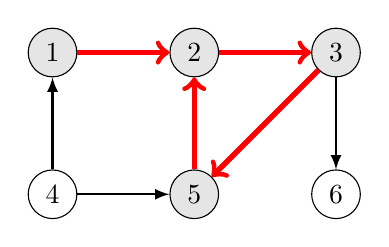
\begin{tikzpicture}[scale=0.9]
\node[draw, circle,fill=gray!20] (1) at (1,5) {$1$};
\node[draw, circle,fill=gray!20] (2) at (3,5) {$2$};
\node[draw, circle,fill=gray!20] (3) at (5,5) {$3$};
\node[draw, circle] (4) at (1,3) {$4$};
\node[draw, circle,fill=gray!20] (5) at (3,3) {$5$};
\node[draw, circle] (6) at (5,3) {$6$};

\path[draw,thick,->,>=latex] (4) -- (1);
\path[draw,thick,->,>=latex] (4) -- (5);
\path[draw,thick,->,>=latex] (3) -- (6);

\path[draw=red,thick,->,line width=2pt] (1) -- (2);
\path[draw=red,thick,->,line width=2pt] (2) -- (3);
\path[draw=red,thick,->,line width=2pt] (3) -- (5);
\path[draw=red,thick,->,line width=2pt] (5) -- (2);
\end{tikzpicture}
\end{center}

探索は状態が1であるノード2に到達しました。
つまり、グラフが閉路を含むということです。
この例では、$2 \rightarrow 3 \rightarrow 5 \rightarrow 2$という閉路が存在します。

\section{木DP  - Dynamic programming}

有向グラフがサイクルを含まないのであれば動的計画法を木上で適用することができます。
例えば、始点ノードから終点ノードへの経路に関する次のような問題を効率的に解くことができます。

\begin{itemize}
\item パスの種類は?
\item 最短あるいは最大のパスは?
\item 最短あるいは最大の辺の数は?
\item 全てのパスにおいて必ず通るノードはあるか?
\end{itemize}

\subsubsection{パス数のカウント}

次のグラフで1から6のパスの数を考えます。

\begin{center}
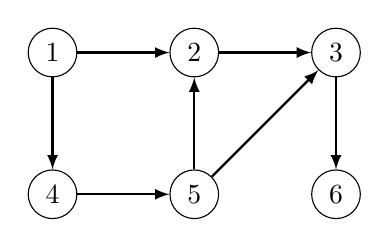
\begin{tikzpicture}[scale=0.9]
\node[draw, circle] (1) at (1,5) {$1$};
\node[draw, circle] (2) at (3,5) {$2$};
\node[draw, circle] (3) at (5,5) {$3$};
\node[draw, circle] (4) at (1,3) {$4$};
\node[draw, circle] (5) at (3,3) {$5$};
\node[draw, circle] (6) at (5,3) {$6$};

\path[draw,thick,->,>=latex] (1) -- (2);
\path[draw,thick,->,>=latex] (2) -- (3);
\path[draw,thick,->,>=latex] (1) -- (4);
\path[draw,thick,->,>=latex] (4) -- (5);
\path[draw,thick,->,>=latex] (5) -- (2);
\path[draw,thick,->,>=latex] (5) -- (3);
\path[draw,thick,->,>=latex] (3) -- (6);
\end{tikzpicture}
\end{center}
このようなパスは以下の3つがあります。
\begin{itemize}
\item $1 \rightarrow 2 \rightarrow 3 \rightarrow 6$
\item $1 \rightarrow 4 \rightarrow 5 \rightarrow 2 \rightarrow 3 \rightarrow 6$
\item $1 \rightarrow 4 \rightarrow 5 \rightarrow 3 \rightarrow 6$
\end{itemize}

$\texttt{paths}(1)=1$です。
$\texttt{paths}(x)$は以下のように再帰的に求めていきます。
\[\texttt{paths}(x) = \texttt{paths}(a_1)+\texttt{paths}(a_2)+\cdots+\texttt{paths}(a_k)\]
は$x$への辺が存在するノードです。
グラフは閉路を持たないため、
$path(x)$の値はトポロジカルソートの順に計算することができます。
上のグラフのトポロジカルソートの1つは以下の通りです。
\begin{center}
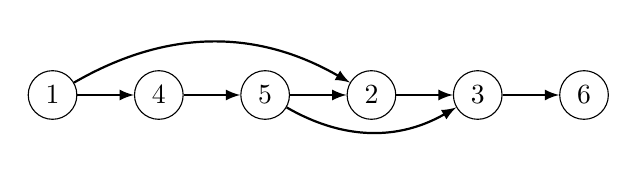
\begin{tikzpicture}[scale=0.9]
\node[draw, circle] (1) at (0,0) {$1$};
\node[draw, circle] (2) at (4.5,0) {$2$};
\node[draw, circle] (3) at (6,0) {$3$};
\node[draw, circle] (4) at (1.5,0) {$4$};
\node[draw, circle] (5) at (3,0) {$5$};
\node[draw, circle] (6) at (7.5,0) {$6$};

\path[draw,thick,->,>=latex] (1) edge [bend left=30] (2);
\path[draw,thick,->,>=latex] (2) -- (3);
\path[draw,thick,->,>=latex] (1) -- (4);
\path[draw,thick,->,>=latex] (4) -- (5);
\path[draw,thick,->,>=latex] (5) -- (2);
\path[draw,thick,->,>=latex] (5) edge [bend right=30] (3);
\path[draw,thick,->,>=latex] (3) -- (6);
\end{tikzpicture}
\end{center}
このためパス数は以下のように求められます。
\begin{center}
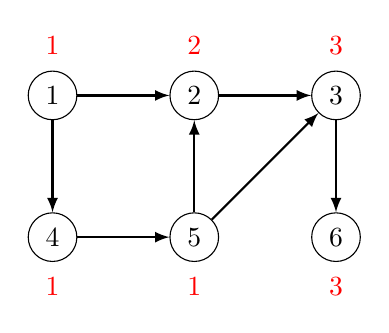
\begin{tikzpicture}[scale=0.9]
\node[draw, circle] (1) at (1,5) {$1$};
\node[draw, circle] (2) at (3,5) {$2$};
\node[draw, circle] (3) at (5,5) {$3$};
\node[draw, circle] (4) at (1,3) {$4$};
\node[draw, circle] (5) at (3,3) {$5$};
\node[draw, circle] (6) at (5,3) {$6$};

\path[draw,thick,->,>=latex] (1) -- (2);
\path[draw,thick,->,>=latex] (2) -- (3);
\path[draw,thick,->,>=latex] (1) -- (4);
\path[draw,thick,->,>=latex] (4) -- (5);
\path[draw,thick,->,>=latex] (5) -- (2);
\path[draw,thick,->,>=latex] (5) -- (3);
\path[draw,thick,->,>=latex] (3) -- (6);

\node[color=red] at (1,2.3) {$1$};
\node[color=red] at (3,2.3) {$1$};
\node[color=red] at (5,2.3) {$3$};
\node[color=red] at (1,5.7) {$1$};
\node[color=red] at (3,5.7) {$2$};
\node[color=red] at (5,5.7) {$3$};
\end{tikzpicture}
\end{center}

$\texttt{paths}(3)$を求める時、ノード2と5からノード3への辺があるので、
$\texttt{paths}(2)+\texttt{paths}(5)$を計算します。
$\texttt{paths}(2)=2$, $\texttt{paths}(5)=1$ですから、$\texttt{paths}(3)=3$となります。

\subsubsection{ダイクストラのアルゴリズムの拡張}

\index{ダイクストラアルゴリズム}

ダイクストラのアルゴリズムを利用すると、
開始ノードから各ノードへの最短経路を使用してそのノードに到達する可能性を示す有向の閉路が存在しないグラフを得ることができます。
このグラフに対しては動的計画法を適用することができます。以下を考えます。
\begin{center}
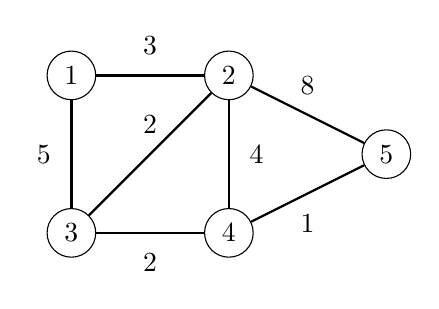
\begin{tikzpicture}
\node[draw, circle] (1) at (0,0) {$1$};
\node[draw, circle] (2) at (2,0) {$2$};
\node[draw, circle] (3) at (0,-2) {$3$};
\node[draw, circle] (4) at (2,-2) {$4$};
\node[draw, circle] (5) at (4,-1) {$5$};

\path[draw,thick,-] (1) -- node[font=\small,label=above:3] {} (2);
\path[draw,thick,-] (1) -- node[font=\small,label=left:5] {} (3);
\path[draw,thick,-] (2) -- node[font=\small,label=right:4] {} (4);
\path[draw,thick,-] (2) -- node[font=\small,label=above:8] {} (5);
\path[draw,thick,-] (3) -- node[font=\small,label=below:2] {} (4);
\path[draw,thick,-] (4) -- node[font=\small,label=below:1] {} (5);
\path[draw,thick,-] (2) -- node[font=\small,label=above:2] {} (3);
\end{tikzpicture}
\end{center}
ノード1からの最短経路は以下のようになります。
\begin{center}
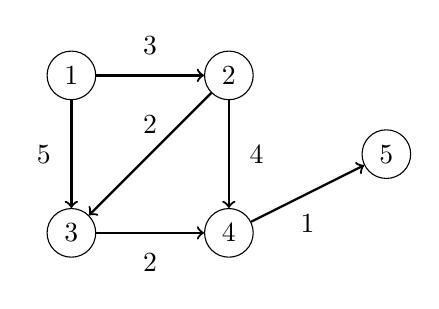
\begin{tikzpicture}
\node[draw, circle] (1) at (0,0) {$1$};
\node[draw, circle] (2) at (2,0) {$2$};
\node[draw, circle] (3) at (0,-2) {$3$};
\node[draw, circle] (4) at (2,-2) {$4$};
\node[draw, circle] (5) at (4,-1) {$5$};

\path[draw,thick,->] (1) -- node[font=\small,label=above:3] {} (2);
\path[draw,thick,->] (1) -- node[font=\small,label=left:5] {} (3);
\path[draw,thick,->] (2) -- node[font=\small,label=right:4] {} (4);
\path[draw,thick,->] (3) -- node[font=\small,label=below:2] {} (4);
\path[draw,thick,->] (4) -- node[font=\small,label=below:1] {} (5);
\path[draw,thick,->] (2) -- node[font=\small,label=above:2] {} (3);
\end{tikzpicture}
\end{center}

これでノード1から5までの最短経路を以下のように求めることができます。
\begin{center}
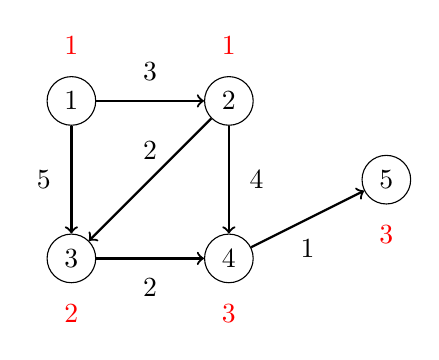
\begin{tikzpicture}
\node[draw, circle] (1) at (0,0) {$1$};
\node[draw, circle] (2) at (2,0) {$2$};
\node[draw, circle] (3) at (0,-2) {$3$};
\node[draw, circle] (4) at (2,-2) {$4$};
\node[draw, circle] (5) at (4,-1) {$5$};

\path[draw,thick,->] (1) -- node[font=\small,label=above:3] {} (2);
\path[draw,thick,->] (1) -- node[font=\small,label=left:5] {} (3);
\path[draw,thick,->] (2) -- node[font=\small,label=right:4] {} (4);
\path[draw,thick,->] (3) -- node[font=\small,label=below:2] {} (4);
\path[draw,thick,->] (4) -- node[font=\small,label=below:1] {} (5);
\path[draw,thick,->] (2) -- node[font=\small,label=above:2] {} (3);

\node[color=red] at (0,0.7) {$1$};
\node[color=red] at (2,0.7) {$1$};
\node[color=red] at (0,-2.7) {$2$};
\node[color=red] at (2,-2.7) {$3$};
\node[color=red] at (4,-1.7) {$3$};
\end{tikzpicture}
\end{center}

\subsubsection{グラフによる問題表現 - Representing problems as graphs}

動的計画問題は閉路が存在しない有向のグラフで表現することができます。
このようなグラフでは、各ノードが動的計画法の状態に対応し、
辺は状態各ノードの依存を示します。

例として,硬貨$\{c_1,c_2,\ldots,c_k\}$を用いて金額$n$を作る問題を考えます。
この問題では,各ノードが金額に対応し,エッジがコインの選び方を示すグラフと捉えることができます。
たとえば,コイン $\{1,3,4\}$ と $n = 6$ の場合, グラフは次のようになります。

\begin{center}
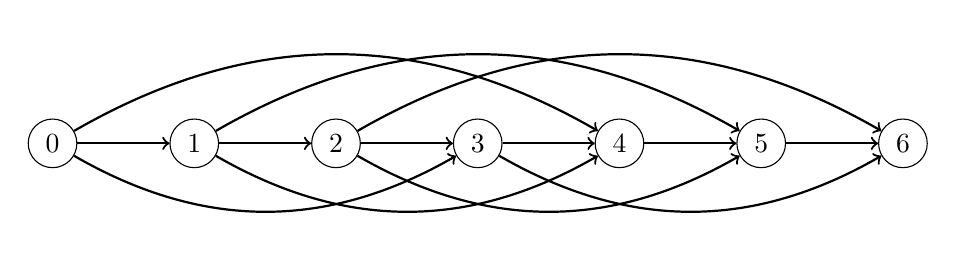
\begin{tikzpicture}[scale=0.9]
\node[draw, circle] (0) at (0,0) {$0$};
\node[draw, circle] (1) at (2,0) {$1$};
\node[draw, circle] (2) at (4,0) {$2$};
\node[draw, circle] (3) at (6,0) {$3$};
\node[draw, circle] (4) at (8,0) {$4$};
\node[draw, circle] (5) at (10,0) {$5$};
\node[draw, circle] (6) at (12,0) {$6$};

\path[draw,thick,->] (0) -- (1);
\path[draw,thick,->] (1) -- (2);
\path[draw,thick,->] (2) -- (3);
\path[draw,thick,->] (3) -- (4);
\path[draw,thick,->] (4) -- (5);
\path[draw,thick,->] (5) -- (6);

\path[draw,thick,->] (0) edge [bend right=30] (3);
\path[draw,thick,->] (1) edge [bend right=30] (4);
\path[draw,thick,->] (2) edge [bend right=30] (5);
\path[draw,thick,->] (3) edge [bend right=30] (6);

\path[draw,thick,->] (0) edge [bend left=30] (4);
\path[draw,thick,->] (1) edge [bend left=30] (5);
\path[draw,thick,->] (2) edge [bend left=30] (6);
\end{tikzpicture}
\end{center}

この表し方をするとノード$0$からノード$n$までの最短経路はコインの枚数が最小の解に対応していることとなり、
ノード$0$からノード$n$までの経路の総数は解の総数に等しくなります。

\section{サクセスパス - Successor paths}

\index{サクセスグラフ - successor graph}
\index{functional graph}

\key{successor graphs}に焦点を当てていきます。
このグラフでは、各ノードの出次辺は1、つまり、ちょうど1本の辺が各ノードから出ています。
サクセスグラフは1つ以上のコンポーネントとからなます。
それぞれのコンポーネントには1つのサイクルとそれにつながるパスがあります。
サクセスグラフはfunctionalグラフと呼ばれることもあります。
これはサクセスグラフがグラフの辺を定義する関数に対応するからです。
関数のパラメータはグラフのノードであり、関数はそのノードの後ろの後ろ、と考えます。

例えば以下の関数を考えます。
\begin{center}
\begin{tabular}{r|rrrrrrrrr}
$x$ & 1 & 2 & 3 & 4 & 5 & 6 & 7 & 8 & 9 \\
\hline
$\texttt{succ}(x)$ & 3 & 5 & 7 & 6 & 2 & 2 & 1 & 6 & 3 \\
\end{tabular}
\end{center}
これは次のようなパスと考えられます。
\begin{center}
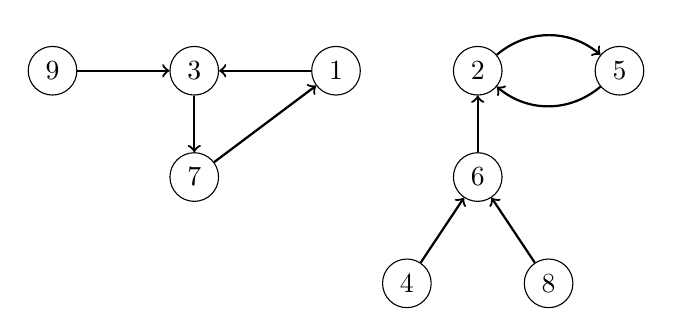
\begin{tikzpicture}[scale=0.9]
\node[draw, circle] (1) at (0,0) {$1$};
\node[draw, circle] (2) at (2,0) {$2$};
\node[draw, circle] (3) at (-2,0) {$3$};
\node[draw, circle] (4) at (1,-3) {$4$};
\node[draw, circle] (5) at (4,0) {$5$};
\node[draw, circle] (6) at (2,-1.5) {$6$};
\node[draw, circle] (7) at (-2,-1.5) {$7$};
\node[draw, circle] (8) at (3,-3) {$8$};
\node[draw, circle] (9) at (-4,0) {$9$};

\path[draw,thick,->] (1) -- (3);
\path[draw,thick,->] (2)  edge [bend left=40] (5);
\path[draw,thick,->] (3) -- (7);
\path[draw,thick,->] (4) -- (6);
\path[draw,thick,->] (5)  edge [bend left=40] (2);
\path[draw,thick,->] (6) -- (2);
\path[draw,thick,->] (7) -- (1);
\path[draw,thick,->] (8) -- (6);
\path[draw,thick,->] (9) -- (3);
\end{tikzpicture}
\end{center}

successorグラフの各ノードは一意な次のノードを持つので、
ノード$x$から始めて$k$歩進んで到達するノードを与える
関数$\texttt{succ}(x,k)$を定義することができます。
たとえば,上のグラフでは $\texttt{succ}(4,6)=2$ で、これは
ノード4から6回移動するとノード2に到達することを表します。
\begin{center}
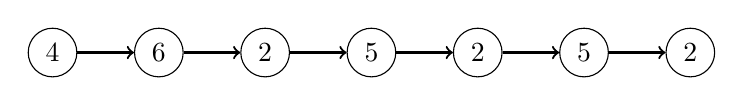
\begin{tikzpicture}[scale=0.9]
\node[draw, circle] (1) at (0,0) {$4$};
\node[draw, circle] (2) at (1.5,0) {$6$};
\node[draw, circle] (3) at (3,0) {$2$};
\node[draw, circle] (4) at (4.5,0) {$5$};
\node[draw, circle] (5) at (6,0) {$2$};
\node[draw, circle] (6) at (7.5,0) {$5$};
\node[draw, circle] (7) at (9,0) {$2$};

\path[draw,thick,->] (1) -- (2);
\path[draw,thick,->] (2) -- (3);
\path[draw,thick,->] (3) -- (4);
\path[draw,thick,->] (4) -- (5);
\path[draw,thick,->] (5) -- (6);
\path[draw,thick,->] (6) -- (7);
\end{tikzpicture}
\end{center}

$\texttt{succ}(x,k)$値を計算する簡単な方法は、ノード$x$から始めて$k$歩を実際に進むことですが、
これには$O(k)$個の時間がかかってしまいます。
前処理を行うことと$O(\log k)$で計算することができます。

この方法を紹介します。$k$が2の累乗であって、最大でも$u$である$\texttt{succ}(x,k)$のすべての値を
事前に計算します。$u$は必要となる最大の数です。
これは以下のような再起的な方法で求めることができます。 

\begin{equation*}
    \texttt{succ}(x,k) = \begin{cases}
               \texttt{succ}(x)              & k = 1\\
               \texttt{succ}(\texttt{succ}(x,k/2),k/2)   & k > 1\\
           \end{cases}
\end{equation*}

各ノードに対して$O(\log u)$個の値を計算するため、
値の事前計算には$O(n \log u)$個の時間がかかります。

\begin{center}
\begin{tabular}{r|rrrrrrrrr}
$x$ & 1 & 2 & 3 & 4 & 5 & 6 & 7 & 8 & 9 \\
\hline
$\texttt{succ}(x,1)$ & 3 & 5 & 7 & 6 & 2 & 2 & 1 & 6 & 3 \\
$\texttt{succ}(x,2)$ & 7 & 2 & 1 & 2 & 5 & 5 & 3 & 2 & 7 \\
$\texttt{succ}(x,4)$ & 3 & 2 & 7 & 2 & 5 & 5 & 1 & 2 & 3 \\
$\texttt{succ}(x,8)$ & 7 & 2 & 1 & 2 & 5 & 5 & 3 & 2 & 7 \\
$\cdots$ \\
\end{tabular}
\end{center}

この事前計算を用いるとステップ数kを2の累乗の和で表すことで、
$\texttt{succ}(x,k)$の任意の値を算出することができます。
例えば、$\texttt{succ}(x,11)$の値を計算したい場合は、
$11 = 8 + 2 + 1$とします。こうすることで、

\[\texttt{succ}(x,11)=\texttt{succ}(\texttt{succ}(\texttt{succ}(x,8),2),1).\]
これは次のように展開されます。
\[\texttt{succ}(4,11)=\texttt{succ}(\texttt{succ}(\texttt{succ}(4,8),2),1)=5.\]

これによって全ての数は$O(\log k)$で求めることができます。
(訳註:ダブリングと呼ばれるテクニックです)

\section{閉路検出 - Cycle detection}

\index{cycle}
\index{閉路検出 - cycle detection}

閉路で終わる有向グラフを考えます。
始点から歩き始めたときに閉路の最初のノードは何でサイクルはいくつのノードを含むか?に焦点をあてます。
\begin{center}
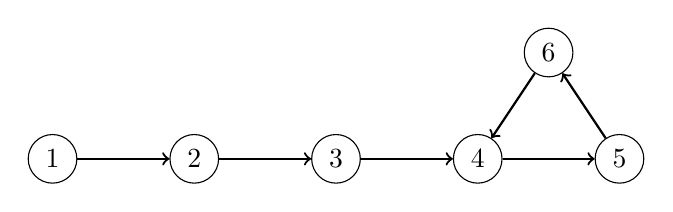
\begin{tikzpicture}[scale=0.9]
\node[draw, circle] (5) at (0,0) {$5$};
\node[draw, circle] (4) at (-2,0) {$4$};
\node[draw, circle] (6) at (-1,1.5) {$6$};
\node[draw, circle] (3) at (-4,0) {$3$};
\node[draw, circle] (2) at (-6,0) {$2$};
\node[draw, circle] (1) at (-8,0) {$1$};

\path[draw,thick,->] (1) -- (2);
\path[draw,thick,->] (2) -- (3);
\path[draw,thick,->] (3) -- (4);
\path[draw,thick,->] (4) -- (5);
\path[draw,thick,->] (5) -- (6);
\path[draw,thick,->] (6) -- (4);
\end{tikzpicture}
\end{center}

ノード1から歩き始めたときに閉路に属する最初のノードは4で、
この閉路は3つのノード(4、5、6)から構成されています。
閉路を検出する簡単な方法は、グラフ内を順に探索していき訪問済みかを記録しておくことです。
あるノードに2度目に達した時にそのノードは閉路に属するの最初のノードです。
この方法は$O(n)$で動作します。

ここで閉路検出のための空間計算量が$O(1)$であるフロイドの循環検出アルゴリズムを紹介します。

\subsubsection{フロイドの循環検出アルゴリズム - Floyd's algorithm}

\index{フロイドの循環検出アルゴリズム - Floyd's algorithm}

\key{フロイドの循環検出アルゴリズム - Floyd's algorithm}とは
\footnote{The idea of the algorithm is mentioned in \cite{knu982}
and attributed to R. W. Floyd; however, it is not known if Floyd actually
discovered the algorithm.}
2つのポインタ$a$、$b$を用いてグラフを探索していく方法です。
両ポインタはグラフの始点であるノードxに位置します。
そして、1ターンごとに、ポインタ$a$は1歩、ポインタ$b$は2歩前進させていきます。
これを両方のポインタが(開始時点を除いて)最初に同じ位置に重なるまで続けます。

\begin{lstlisting}
a = succ(x);
b = succ(succ(x));
while (a != b) {
    a = succ(a);
    b = succ(succ(b));
}
\end{lstlisting}


$k$歩で出会った時、ポインタ$a$は$k$歩、ポインタ$b$は$2k$歩歩いているので、
閉路の長さは$k$で割ることができます。
このため、$a$をノード$x$に移動して再び$a$と$b$が重なるところまでポインタを進めると閉路に所属する最初のノードを知ることができます。

\begin{lstlisting}
a = x;
while (a != b) {
    a = succ(a);
    b = succ(b);
}
first = a;
\end{lstlisting}

そして、サイクルの長さは以下のように求めることができます。
\begin{lstlisting}
b = succ(a);
length = 1;
while (a != b) {
    b = succ(b);
    length++;
}
\end{lstlisting}